%%% LaTeX Template: Two column article
%%%
%%% Source: http://www.howtotex.com/
%%% Feel free to distribute this template, but please keep to referal to http://www.howtotex.com/ here.
%%% Date: February 2011

%%% Preamble
\documentclass[	DIV=calc,%
							paper=a4,%
							fontsize=11pt,%
							twocolumn]{scrartcl}	 					% KOMA-article class

\usepackage{lipsum}													% Package to create dummy text

\usepackage[english]{babel}										% English language/hyphenation
\usepackage[protrusion=true,expansion=true]{microtype}				% Better typography
\usepackage{amsmath,amsfonts,amsthm}					% Math packages
\usepackage[pdftex]{graphicx}									% Enable pdflatex
\usepackage[svgnames]{xcolor}									% Enabling colors by their 'svgnames'
\usepackage[hang, small,labelfont=bf,up,textfont=it,up]{caption}	% Custom captions under/above floats
\usepackage{epstopdf}												% Converts .eps to .pdf
\usepackage{subfig}													% Subfigures
\usepackage{booktabs}												% Nicer tables
\usepackage{fix-cm}													% Custom fontsizes



%%% Custom sectioning (sectsty package)
\usepackage{sectsty}													% Custom sectioning (see below)
\allsectionsfont{%															% Change font of al section commands
	\usefont{OT1}{phv}{b}{n}%										% bch-b-n: CharterBT-Bold font
	}

\sectionfont{%																% Change font of \section command
	\usefont{OT1}{phv}{b}{n}%										% bch-b-n: CharterBT-Bold font
	}



%%% Headers and footers
\usepackage{fancyhdr}												% Needed to define custom headers/footers
	\pagestyle{fancy}														% Enabling the custom headers/footers
\usepackage{lastpage}	

% Header (empty)
\lhead{}
\chead{}
\rhead{}
% Footer (you may change this to your own needs)
\lfoot{\footnotesize \texttt{http://proactive.activeeon.com/} \textbullet ~Big Data Landscape}
\cfoot{}
\rfoot{\footnotesize page \thepage\ of \pageref{LastPage}}	% "Page 1 of 2"
\renewcommand{\headrulewidth}{0.0pt}
\renewcommand{\footrulewidth}{0.4pt}



%%% Creating an initial of the very first character of the content
\usepackage{lettrine}
\newcommand{\initial}[1]{%
     \lettrine[lines=3,lhang=0.3,nindent=0em]{
     				\color{DarkBlue}
     				{\textsf{#1}}}{}}



%%% Title, author and date metadata
\usepackage{titling}															% For custom titles

\newcommand{\HorRule}{\color{DarkBlue}%			% Creating a horizontal rule
									  	\rule{\linewidth}{1pt}%
										}

\pretitle{\vspace{-30pt} \begin{flushleft} \HorRule 
				\fontsize{50}{50} \usefont{OT1}{phv}{b}{n} \color{DarkOrange} \selectfont 
				}
\title{Big Data Landscape}					% Title of your article goes here
\posttitle{\par\end{flushleft}\vskip 0.5em}

\preauthor{\begin{flushleft}
					\large \lineskip 0.5em \usefont{OT1}{phv}{b}{sl} \color{DarkOrange}}
\author{Ge Song, Nicolas Narbais, }											% Author name goes here
\postauthor{\footnotesize \usefont{OT1}{phv}{m}{sl} \color{DarkBlue} 
					ActiveEon 								% Institution of author
					\par\end{flushleft}\HorRule}

\date{}																				% No date



%%% Begin document
\begin{document}
\maketitle
\thispagestyle{fancy} 			% Enabling the custom headers/footers for the first page 
% The first character should be within \initial{}
\initial{E}\textbf{xecutive Summary: }


\section*{\color{DarkOrange}Introduction}

\subsection*{Challenges of Big Data processing}

\subsection*{Real-time processing for data streams}
 

\section*{\color{DarkOrange}Parallel Data Processing}

\initial{P}arallel computing is a computation model which uses two or more processors (cores or computers) in combination to perform multiple operations concurrently. The basic condition for parallel computing is that in general, a large problem can be divided into a limited number of smaller problems, and these smaller problems can be handled simultaneously.
					
Unlike the traditional serial computation, parallel computing uses multiple resources simultaneously to solve a problem. The problem should first be cut into a series of instructions, which will later be executed simultaneously on different processors. This model is much more suitable for explaining, modeling and solving complex real world phenomena. It does not only speed up the time spent to perform a large task, but also makes it possible to process large-scale data sets or complex problems which cannot be handled by a single machine.
					
In parallel computing, there are mainly two forms of parallelism: 
\begin{itemize}
\item Data Parallelism

\item Task Parallelism

\end{itemize}
					
We will introduce them separately in the coming section. 

\subsection*{Two types of parallelisms}

\textbf{Data parallelism} focuses on distributing data across different parallel computing resources, in which the same computation is applied to multiple pieces of data. This is usually used for data-intensive tasks. Fig. \ref{fig:data_para} shows the schematic of data parallelism.

\begin{figure}
  \centering
    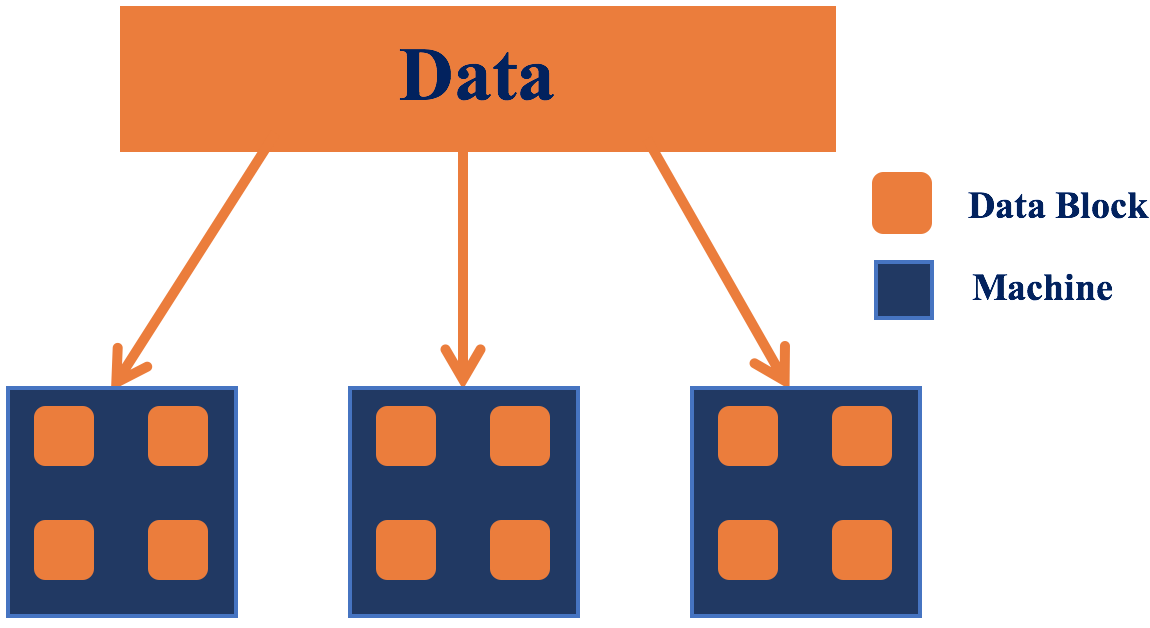
\includegraphics[width=0.4\textwidth]{images/data_para.png}
    \caption{Data Parallelism Schematic}
    \label{fig:data_para}   
\end{figure}

In a data parallelism process, the data set is first divided into partitions, which will later be processed by different processors using the same task. This simple idea makes the storing and handling of big data possible. For example, Facebook has several million photos uploaded each day. But these photos are too large to be stored in a single machine. Then a data parallelism strategy is suitable for this problem.

However, because each machine only has a subset of data, gathering the results together is a problem that this model needs to address. At the same time, the main factor affecting the performance of this model is the transmission of intermediate data, hence reducing the amount of data to be transferred is another problem to face.
Since data parallelism emphasizes the parallel and distributed nature of data, when the size of data is growing, it is inevitable to use this model in parallel computing. Examples of Big Data frameworks that uses data parallelism are: Hadoop MapReduce \cite{1}, Apache Spark\cite{2}, YARN\cite{3}, and Apache Storm\cite{4}.

\textbf{Task parallelism} focuses on distributing tasks concretely performed by processors across different parallel computing resources, in which the same data (or maybe different data in a hybrid system) is processed by different tasks. This is usually used for computation-intensive tasks.

In a task parallelism process, the parallelism is organized around the functions to be run rather than around the data. It depends on task decomposition. This idea makes it possible to handle a complex problem. 
%For example, in a semantic join, task 1 needs to save the data which meets a certain condition in a specific data structure, and task 2 needs to use the data which meets another condition to probe this data structure. This process can be considered as a task parallel process.

The difficulties of this type of process lie first on the decomposition of the work, specifically the decomposition of queries in a join process. Also task parallelism processes usually suffer from bad load balancing, since it is not easy to divide tasks with equal complexity. The communication among tasks is another problem. Synchronization is the most important communication approach in task parallelism processes, and can be divided into thread synchronization and data synchronization. Thread synchronization focuses on determining the order of execution in order to avoid Data Race Condition problems. Data synchronization is mainly used to ensure the consistency among multiple copies of data.

Recently, the most popular task parallelism example is deep learning. Deep learning is a branch of machine learning which is based on a set of algorithms which attempt to model high-level abstractions in data by using multiple processing layers. The difference between deep learning and traditional machine learning is that in deep learning instead of having one model to train all the data, we separate the model into layers, and each layer can be considered as a sub-task of the whole model.

The most common combination of data parallelism and task parallelism is pipelining. Suppose you have multiple tasks, task I, task II and task III, instead of having each one operating on the data independently, pipelining takes the data and first give it to task I, then task II and finally task III. Image processing often chooses to use a pipeline. Images are coming in a stream, some of the processing starts with the first task, and applies a certain filter on the images, then passes on to the second task, and so on. 
%This is a very common combination of task parallelism and data parallelism. 
An example of pipeline processing of images is shown in Fig. \ref{fig:task_para}.

\begin{figure}
  \centering
    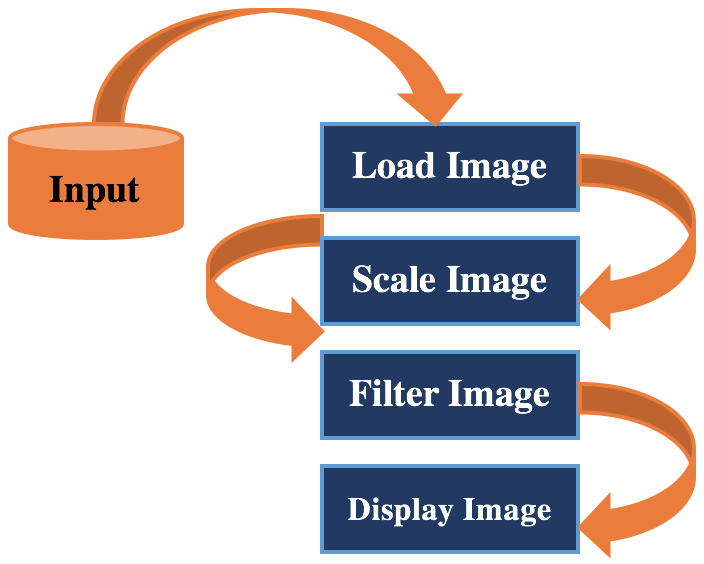
\includegraphics[width=0.4\textwidth]{images/task_para.png}
    \caption{Images Pipeline Processing}
    \label{fig:task_para}   
\end{figure}

Task parallelism and data parallelism complement each other, and they are often used together to tackle large-scale data processing problems. The Big Data frameworks that use task parallelism are: Apache YARN \cite{3} and Apache Storm \cite{4}. They are hybrid systems which support both task and data parallelism.


\subsection*{Big Data processing systems}

\textbf{MapReduce} is a flexible and scalable parallel and distributed programming paradigm which is specially designed for data-intensive processing. It was initially introduced  by Google \cite{Dean:2004:MSD:1251254.1251264} and popularized by the Hadoop framework. 

The concept of MapReduce has been widely known since 1995 with the message passing Interface (MPI) \cite{MPI} standard, having \emph{reduce}  and \emph{scatter} operations. %\footnote{\url{http://mpitutorial.com/tutorials/mpi-reduce-and-allreduce/}} 
 %\footnote{\url{http://mpitutorial.com/tutorials/performing-parallel-rank-with-mpi/}}.
 The MapReduce programming model is composed of a Map procedure and a Reduce procedure. The Map task is usually used for performing some preliminary and cleaning work such as filtering and sorting. For example we can use a Map task to sort the students by alphabetical order of their surname, and then filter the students whose score is below a certain level. The Reduce task is used to perform a summary operation such as count or aggregation. For example we can use a Reduce task to count the number of students whose score is above a given level.  

The idea of the MapReduce paradigm comes from high-order functional programming, where Map and Reduce are two primitives. In this paradigm every record is represented by a $<key, value>$ pair. The Map function processes a fragment of $<key, value>$ pairs in order to generate a list of intermediate $<key, value>$ pairs. Each $<key, value>$ pair is processed by the same map function on different machines without depending on other pairs. The output keys of the Map tasks could be either the same as the input keys or different from them. The output $<key, value>$ pairs have an information of partition which indicates to which Reduce task this pair needs to be sent. The partition information makes sure that all pairs with the same key can be later sent to the same Reduce task. The Reduce function gathers the outputs of the same partition from all map tasks together through a Shuffle phase and merges all the values associated with the same key, then produces a list of $<key, value>$ pairs as output. 

\begin{figure}
  \centering
    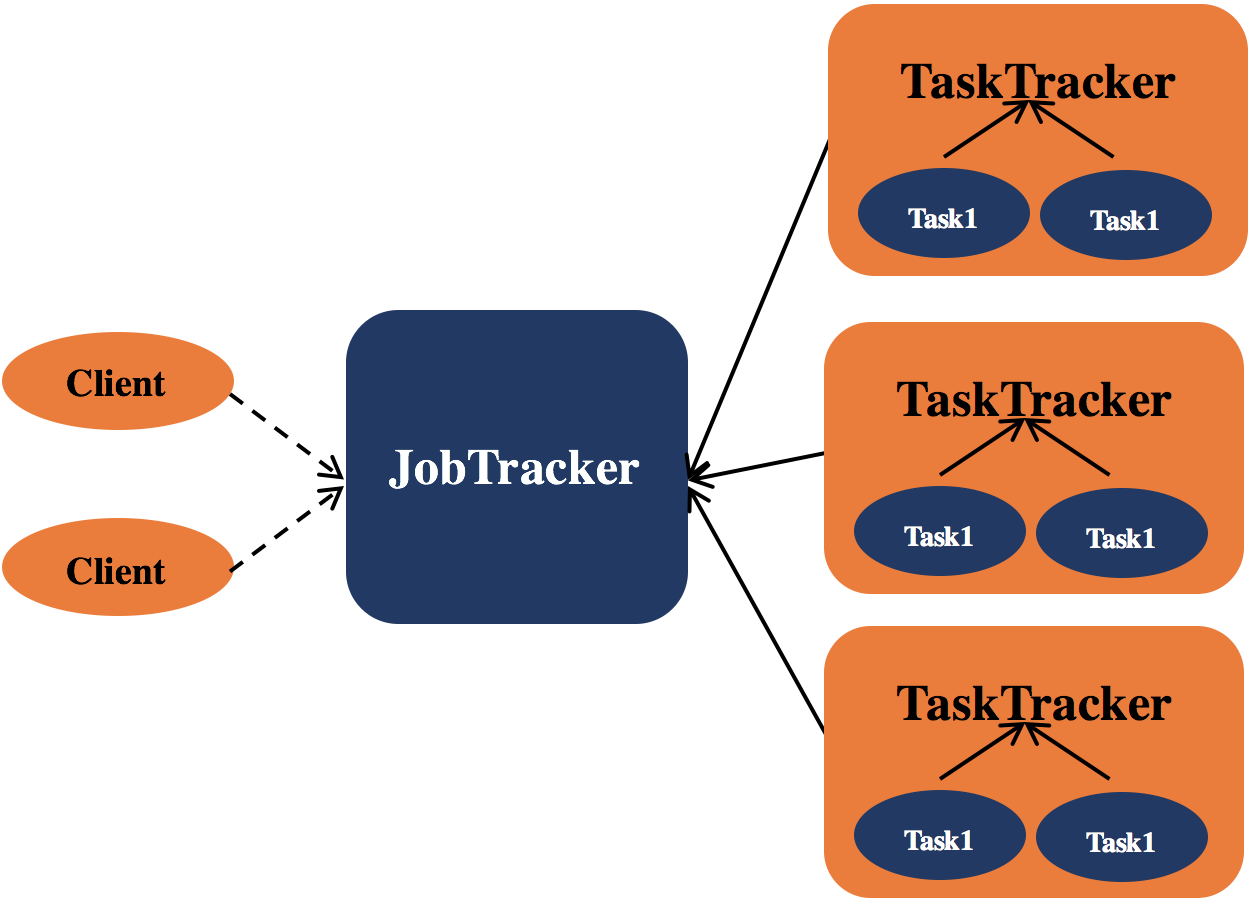
\includegraphics[width=0.4\textwidth]{images/mapreduce.png}
    \caption{Physical Structure of Hadoop System}
    \label{fig:MapReduce0}   
\end{figure}

\textbf{Hadoop} \cite{2} is an open-source framework written in Java for distributed storing and processing large scale data sets. The core of Hadoop contains a distributed storage named Hadoop Distributed File System (HDFS), and the MapReduce programming paradigm. HDFS is a distributed, scalable, and portable file-system written in Java. It stores large files across multiple machines on a cluster. Its reliability is achieved by replicating the data among multiple nodes. The default number of replications is set to 3, which means the same piece of data is stored on three nodes. 
It is very popular not only among the academic institution but also in many companies such as web search, social network, economic computation and so on. A lot of research work focuses on optimizing Hadoop performance and its efficiency in many different aspects.

The whole system of Hadoop works in a master-slave manner, with JobTracker as the master, and the other nodes as slaves. A TaskTracker daemon runs on each slave node. 
The JobTracker daemon is responsible for resource allocation (e.g. managing the worker nodes), tracking (e.g. resource consumption or resource availability) and management (e.g. scheduling). 
The TaskTracker has much more simple responsibilities. It is in charge of launching tasks with an order decided by the JobTracker, and sending the task status information back to JobTracker periodically. The schematic of this process is shown in Fig.~\ref{fig:MapReduce0}.



When running a Hadoop job, input data will first be divided into some splits (64M by default). Then each split will be processed by a user-defined map task. 

So the whole process of a Hadoop job as shown in Fig.~\ref{fig:MapReduce1} can be summarized as follow:

\begin{itemize}

\item \textbf{Step 1:} Split data into blocks (64M by default)

\item \textbf{Step 2:} Map Phase: Extract information from data (filter, sort)

\item \textbf{Step 3:} Shuffle Phase: Exchange data through network from Map Phase to Reduce Phase

\item \textbf{Step 4:} Reduce Phase: Summary operation (count, aggregation)

\end{itemize}


\begin{figure*}
  \centering
    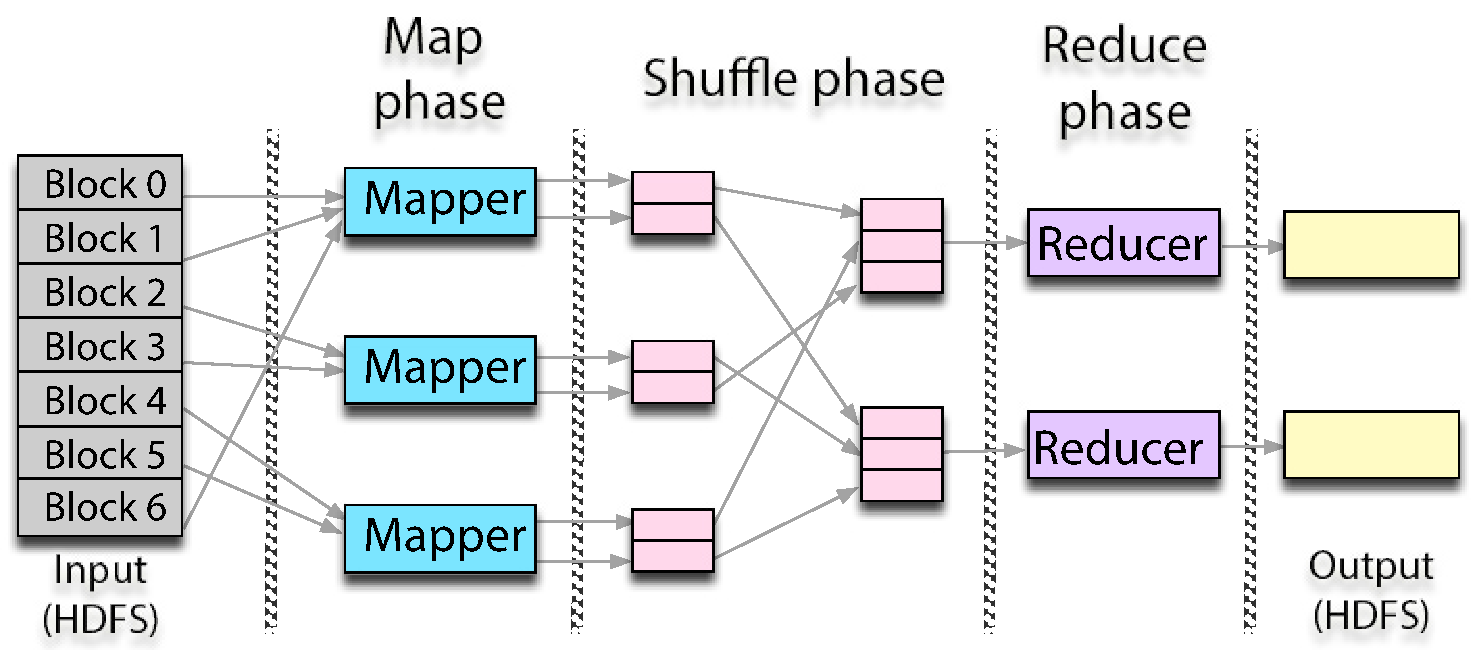
\includegraphics[width=0.8\textwidth]{images/map_reduce.pdf}
    \caption{Logical View of Hadoop Framework}
    \label{fig:MapReduce1}   
\end{figure*}


The previous introduction on Hadoop shows that a Hadoop MapReduce job has some special characteristics as shown below,

\begin{itemize}
\item \textbf{Execution Similarity:} According to the programming model, users only have to provide a map function and a reduce function. And the execution for each Map task (or Reduce task) is very similar to others. In other words, all data will be processed by these functions repeatedly. Thanks to this design, we only need to study how each $<key, value>$ pairs are processed for a particular job, as reading, sorting, transferring and writing data are independent of these two functions.

\item \textbf{Data Similarity:} MapReduce is well suited for off-line batches processing. And it is usually used to do repeated work in which the input data has very similar format, such as log analysis, inverted index and so on. We can just take a look at a small sample and then we can estimate the whole dataset.
\end{itemize}

Hadoop is now a very mature system, with specific application and user groups. However, due to the limitation of the MapReduce paradigm and the Hadoop implementation, it has performance limitations in some application scenarios. In order to better integrate Hadoop in the applications, 
many works have been done from the very beginning to extend Hadoop and to improve its performance. We discuss a limited number of them.

The whole system of Hadoop works in a master-slave manner, with JobTracker as the master, and the other nodes as slaves. A TaskTracker daemon runs on each slave node. The JobTracker daemon is responsible for resource allocation (e.g. managing the worker nodes), tracking (e.g. resource consumption or resource availability) and management (e.g. scheduling). The TaskTracker has much more simple responsibilities. It is in charge of launching tasks with an order decided by the JobTracker, and sending the task status information back to JobTracker periodically. The schematic of this process is shown in Fig. 2.3.
When running a Hadoop job, input data will first be divided into some splits (64M by default). Then each split will be processed by a user-defined map task.
So the whole process of a Hadoop job as shown in Fig. 2.4 can be summarized as follow:

\begin{itemize}

\item \textbf{Step 1:} Split data into blocks (64M by default)

\item \textbf{Step 2:} Map Phase: Extract information from data (filter, sort)

\item \textbf{Step 3:} Shuffle Phase: Exchange data through network from Map Phase to Reduce Phase

\item \textbf{Step 3:} Reduce Phase: Summary operation (count, aggregation)

\end{itemize}

The previous introduction on Hadoop shows that a Hadoop MapReduce job has some
special characteristics as shown below,

\begin{itemize}

\item \textbf{Execution Similarity:} According to the programming model, users only have to provide a map function and a reduce function. And the execution for each Map task (or Reduce task) is very similar to others. In other words, all data will be processed by these functions repeatedly. Thanks to this design, we only need to study how each < key,value > pairs are processed for a particular job, as reading, sorting, transferring and writing data are independent of these two functions.

\item \textbf{Data Similarity:} MapReduce is well suited for off-line batches processing. And it is usually used to do repeated work in which the input data has very similar format, such as log analysis, inverted index and so on. We can just take a look at a small sample and then we can estimate the whole dataset.


\end{itemize}


Hadoop is now a very mature system, with specific application and user groups. However, due to the limitation of the MapReduce paradigm and the Hadoop implementation, it has performance limitations in some application scenarios. In order to better integrate Hadoop in the applications, many works have been done from the very beginning to extend Hadoop and to improve its performance, mainly through the following three ways:

\begin{itemize}

\item Improve the performance of Hadoop by predicting its performance and tuning the parameters.

\item Extend Hadoop to have database-like operations.

\item Combine with other programming language or model.

\end{itemize}

\textbf{Apache Spark} \cite{2} is another popular parallel computing framework after Hadoop MapReduce. Spark provides an application programming interface in Java, Scala, Python and R on a data structure called the resilient distributed dataset (RDD). Spark also uses the MapReduce paradigm but it overcomes the limitations in MapReduce. Hadoop MapReduce forces a particular linear data flow, it reads input data from disk, maps a function across the data, reduces the results of the map, and stores reduction results on disk. The resilient distributed dataset structure works as a working set for distributed programs, it offers a restricted form of distributed shared memory. Unlike Hadoop jobs, the intermediate data of Spark can be saved in memory, which avoids the unnecessary reading and writing from HDFS. Therefore Spark is better for data mining and machine learning algorithms, which require iterations. RDD facilitates the implementation of iterative algorithms which need to visit the dataset multiple times in a loop. It also makes it easy to do interactive or exploratory data analysis, like repeated database-style querying of data.
Spark requires a manager which is in charge of the cluster, and a distributed file system. Spark also supports a pseudo distributed mode (local mode), which is usually needed for testing.

Compared with Hadoop, Spark has the following advantages:

\begin{figure}
  \centering
    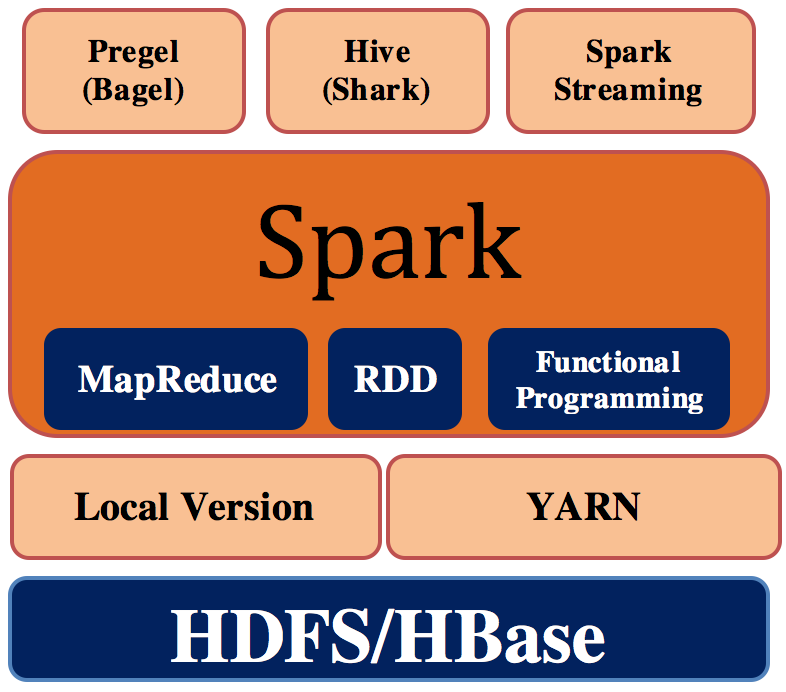
\includegraphics[width=0.5\textwidth]{images/spark.png}
    \caption{Structure of Spark System.}
    \label{fig:Spark}   
\end{figure}

\begin{itemize}

\item Store intermediate data into memory, providing a higher efficiency for iterative opera- tions. So Spark is more suitable for Data Mining and Machine Learning algorithms containing a lot of iterations.

\item Spark is more flexible than Hadoop. It provides many operators like: map, filter, flatMap, sample, groupByKey, reduceByKey, union, join, cogroup, mapValues, sort, partionBy, while Hadoop only provides Map and Reduce. However, due to the char- acteristics of RDD, Spark does not perform well on the fine-grained asynchronous update applications or the applications with incremental changes, such as the web crawlers with updates.

\item By providing a wealth of Scala, Java, Python APIs and interactive Shell API, Spark has a higher availability with different programming languages and different modes to use.

\end{itemize}

According to the characteristics of Spark, its applicable scenarios are:

\begin{itemize}
\item Iterative calculations requiring multiple operations

\item Applications that require multiple operations on a specific data set

\end{itemize}

And the benefit increases with the amount of data and the number of operations. But the benefit is smaller in applications with a small amount of data and intensive computations.
The structure of a Spark system is shown in Fig. \ref{fig:Spark}.

\textbf{YARN} \cite{3} is an attempt to take Apache Hadoop beyond MapReduce for data-processing. As we explained above, in Hadoop, the two major responsibilities of the JobTracker are resource management and job scheduling or monitoring. As there is only one JobTracker in the whole system, it becomes a bottleneck. The fundamental idea of YARN is to split these functions into two separate daemons --- a global ResourceManager (RM) and a per-application ApplicationMaster (AM).

\begin{figure}
  \centering
    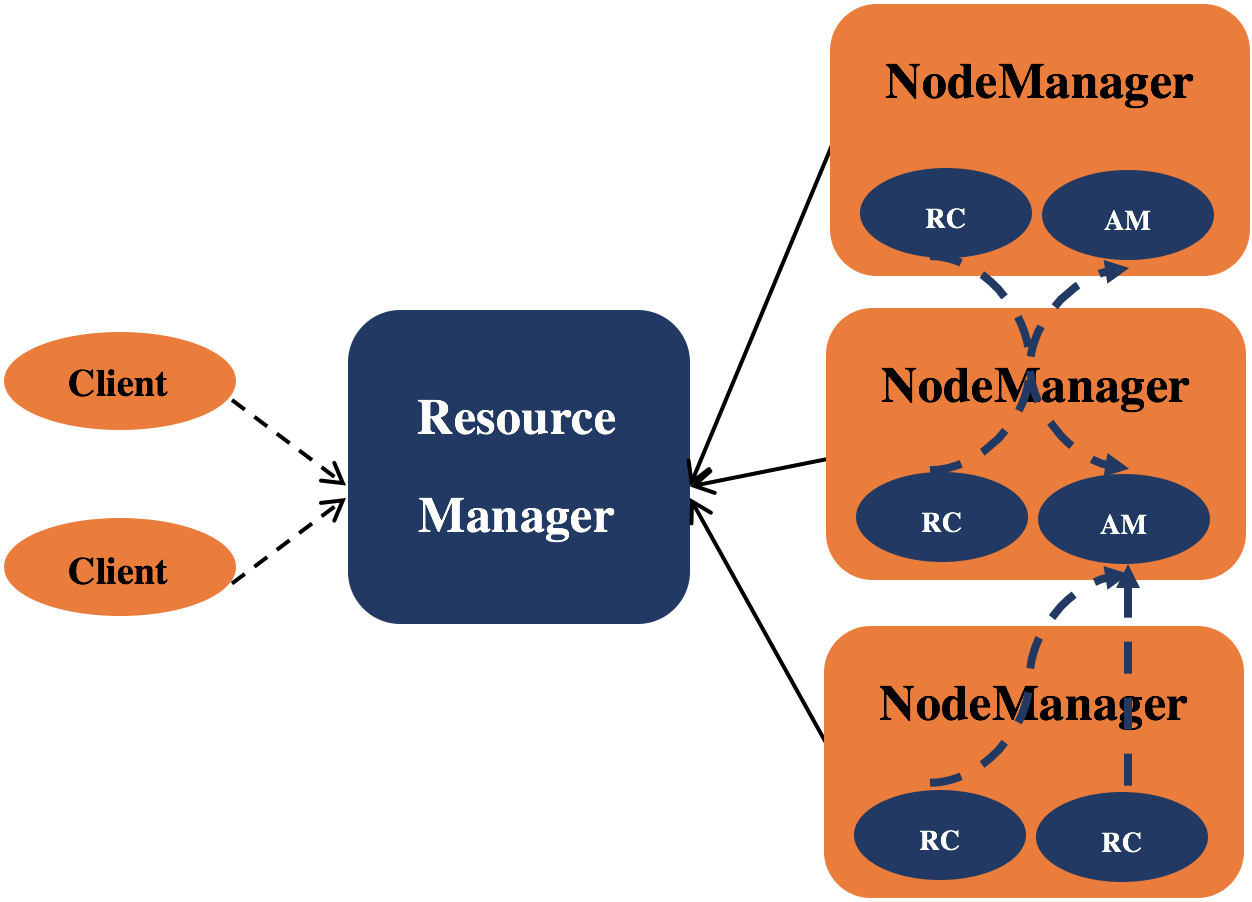
\includegraphics[width=0.4\textwidth]{images/YARN.png}
    \caption{Architectural View of YARN}
    \label{fig:YARN}   
\end{figure}

The ResourceManager together with the per-node slave daemon NodeManger forms a new generic system for managing tasks in a distributed manner. Moreover, the ResourceManager is the ultimate authority that arbitrates resources among all applications in the system, while the per-application ApplicationMaster is a framework specific entity and is used to negotiate resources from the master ResourceManager and the slaves NodeManagers to execute and monitor the tasks. A pluggable Scheduler is used in the ResourceManager to allocate resources to jobs. The Scheduler works using an abstract concept of Resource Container (RC) which incorporates resource elements such as CPU, Memory, Disk, Network etc. The NodeManager is a per-node slave daemon, and its responsibility is to launch the tasks and to monitor the resources (CPU, Memory, Disk, Network). From the system perspective, the ApplicationMaster runs as a normal container.
An architectural view of YARN is shown in Fig.~\ref{fig:YARN}.

\textbf{Hadoop}, \textbf{Spark} and \textbf{YARN} all use the \textbf{MapReduce} paradigm as their abstract computational concept. The ecosystem of MapReduce and its derivative methods are mature and very good for parallel processing of big data. But most of them are still an `offline' processing platform, which means that they can not handle dynamic data streams.



\subsection*{Parallel data warehouse}

\subsection*{ETL for Big Data}


\section*{\color{DarkOrange} Real-time Data Processing}




\subsection*{Rules for Data Stream processing}

\subsection*{Data Stream management systems}

\subsection*{Introduction to Apache Storm}

\section*{\color{DarkOrange} ProActive}

\subsection*{Introduction to ProActive}

\subsection*{Role of ProActive in Big Data area}

\subsection*{Advantages of using ProActive}

\bibliographystyle{unsrt}
\bibliography{biblio}

\end{document}

